\documentclass[12pt,reqno,final]{amsart}
\usepackage[round,numbers,sort&compress]{natbib}
\usepackage{graphicx}
\usepackage{times}
\usepackage{rotating}
\usepackage{subfig}
\usepackage{Sweave}

\title[DEB fitting notes]{Fitting Dynamic Energy Budget Models:
  Parameter Covariation}

\setlength{\textwidth}{6.25in}
\setlength{\textheight}{8.75in}
\setlength{\evensidemargin}{0in}
\setlength{\oddsidemargin}{0in}
\setlength{\topmargin}{-.35in}
\setlength{\parskip}{.1in}
\setlength{\parindent}{0.0in}

\theoremstyle{plain}
\newtheorem{thm}{Theorem}
\newtheorem{corol}[thm]{Corollary}
\newtheorem{prop}[thm]{Proposition}
\newtheorem{lemma}[thm]{Lemma}
\newtheorem{defn}[thm]{Definition}
\newtheorem{hyp}[thm]{Hypothesis}
\newtheorem{example}[thm]{Example}
\newtheorem{conj}[thm]{Conjecture}
\newtheorem{algorithm}[thm]{Algorithm}
\newtheorem{remark}{Remark}
\renewcommand\thethm{\arabic{thm}}
\renewcommand{\theremark}{}

\numberwithin{equation}{part}
\renewcommand\theequation{\arabic{equation}}
\renewcommand\thesection{\arabic{section}}
\renewcommand\thesubsection{\thesection.\arabic{subsection}}
\renewcommand\thefigure{\arabic{figure}}
\renewcommand\thetable{\arabic{table}}
\renewcommand\thefootnote{\arabic{footnote}}

\begin{document}

\maketitle

I have done some initial simulation recovery experiments, and I want
to explore the results of those efforts here. Note that the
correlations among parameters for the four different parameter sets
that have been fitted can be found in
``Correlation\_among\_parameters.pdf''. In this file, I am exploring
the second parameter set, where the correlations were very clear.

I begin by looking at all of the estimated values for the fitted
parameters, plotted as pairwise scatterplots to look for obvious
correlations between the estimates. I focus only on those parameter
sets where the log-likelihood was within 20 units of the minimum
log-likelihood (note that subplex had not converged for \emph{any} of
these parameter sets - yikes). Points colored red are within 5
log-likelihood units of the minimum. I will focus my attention
initially on the energy allocation parameters, and show the energy
ingestion parameters and initial condition parameters next. Note that
$\nu$ is on the logarithmic scale.
\begin{figure}
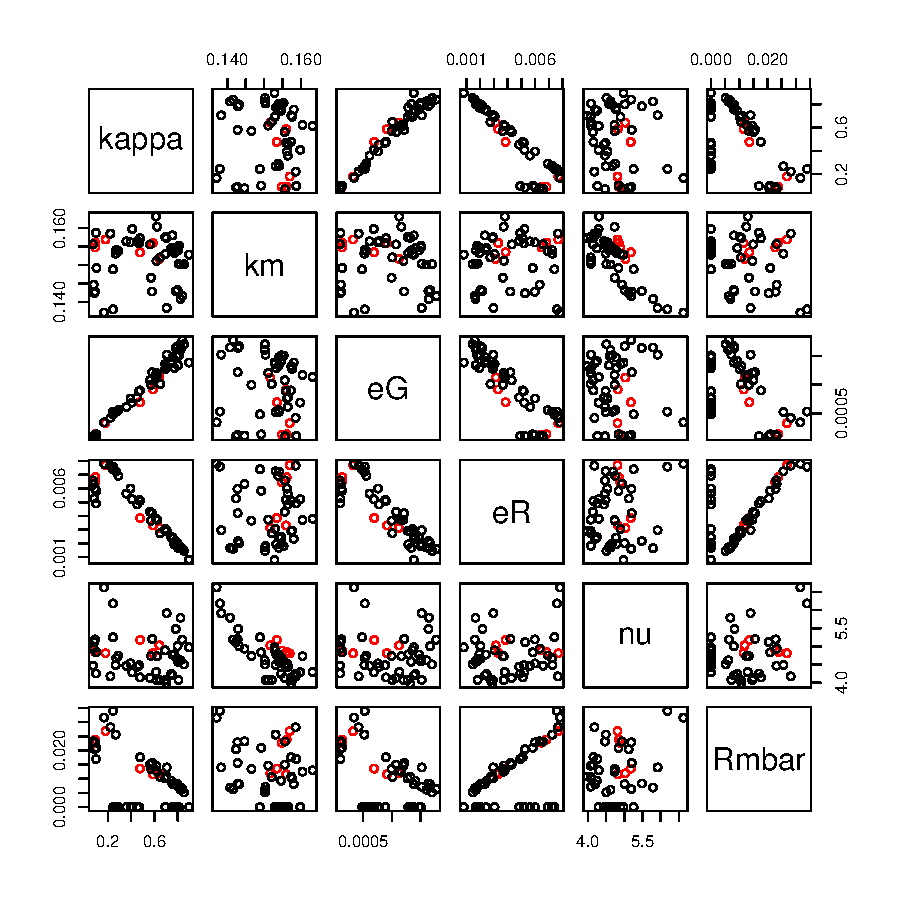
\includegraphics{Solving_the_problem_of_parameter_covariation_4-001}
\end{figure}

These show considerable correlation among the parameters. For example,
the estimate of the energy requirement for maturation $\bar{R_m}$ is
positively correlated with the estimate of the cost of
reproduction $\epsilon_R$, and the cost of growth $\epsilon_G$ is
negatively correlated with the somatic maintenance rate $k_m$. This
correlation is unsurprising, given that the DEB model, like
all biological models, is overparameterized. Morever, the energy
budget creates constraints that may allow parameters to trade-off
against one another, producing similar growth trajectories. It may be
that, although individual parameters cannot be well-estimated, certain
parameter combinations can be, and the model can be reparameterized in
terms of these estimable \emph{compound} parameters.

One big, important difference between the previous parameter set and
this one is the fact that $\nu$ is now reasonably well-estimated. The
range of $\nu$ estimates is 1.9 to 3.98. The difference is that the
truth was 1.8, rather than 18.1. So if $\nu$ is small, the likelihood
surface may not be flat for increasing $\nu$, as it seemed to be
before.

The ingestion parameters are, on the whole, badly identified. Maximum
surface-area specific assimilation rate $p_{am}$ and half-saturation
constant $F_h$ have to be plotted on the log scale to visualize all of
the variation. There appears to be a strong positive correlation
between $p_{am}$ and $F_h$, and between $p_{am}$ and $e_A$.

\begin{figure}
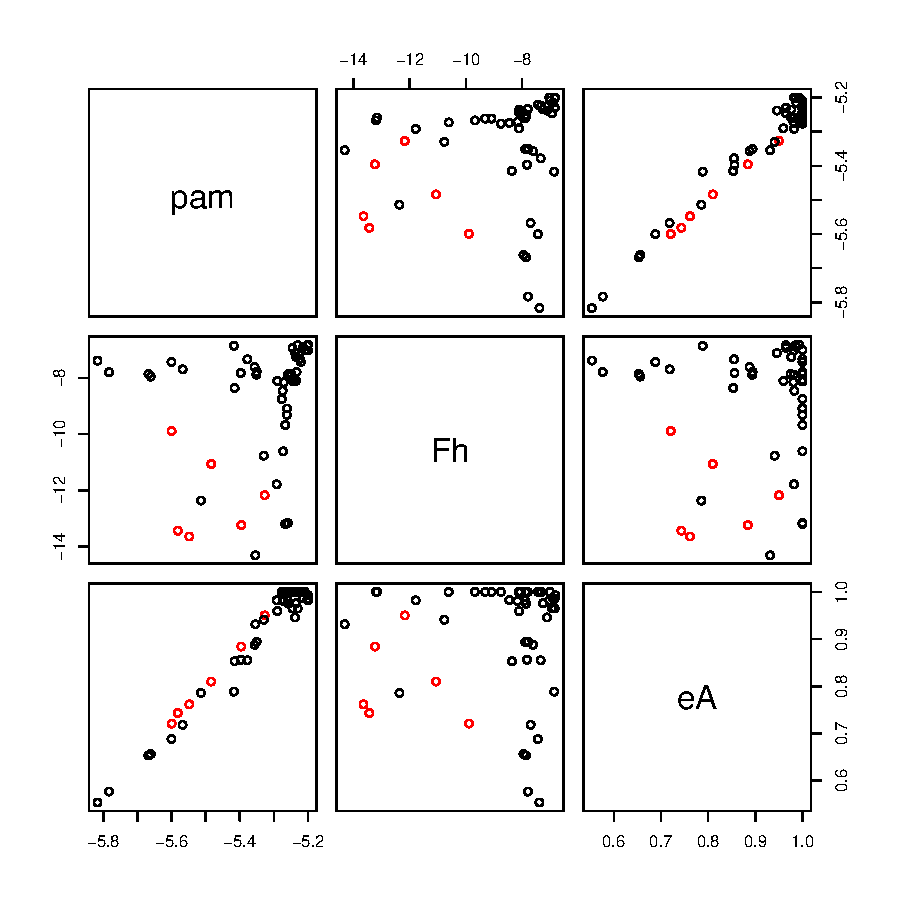
\includegraphics{Solving_the_problem_of_parameter_covariation_4-002}
\end{figure}

Given that the ingestion parameters seem to be difficult to estimate,
a problem that is unsurprising given that we are only considering data
at a single food level, I will focus my attention on the energy
allocation parameters only.

Let's first look at the estimates for each parameter by creating a
histogram of the ratio of the estimates to the true value - a
histogram with peak at, or near, unity inidicates that the parameter
was well-estimated. The red line indicates the truth, the blue line
indicates the mean parameter estimate, and the green line the median
estimate. This will allow us to focus our attention on only those
parameters that might need to be looked as ratios or products with
other parameters.
\begin{figure}
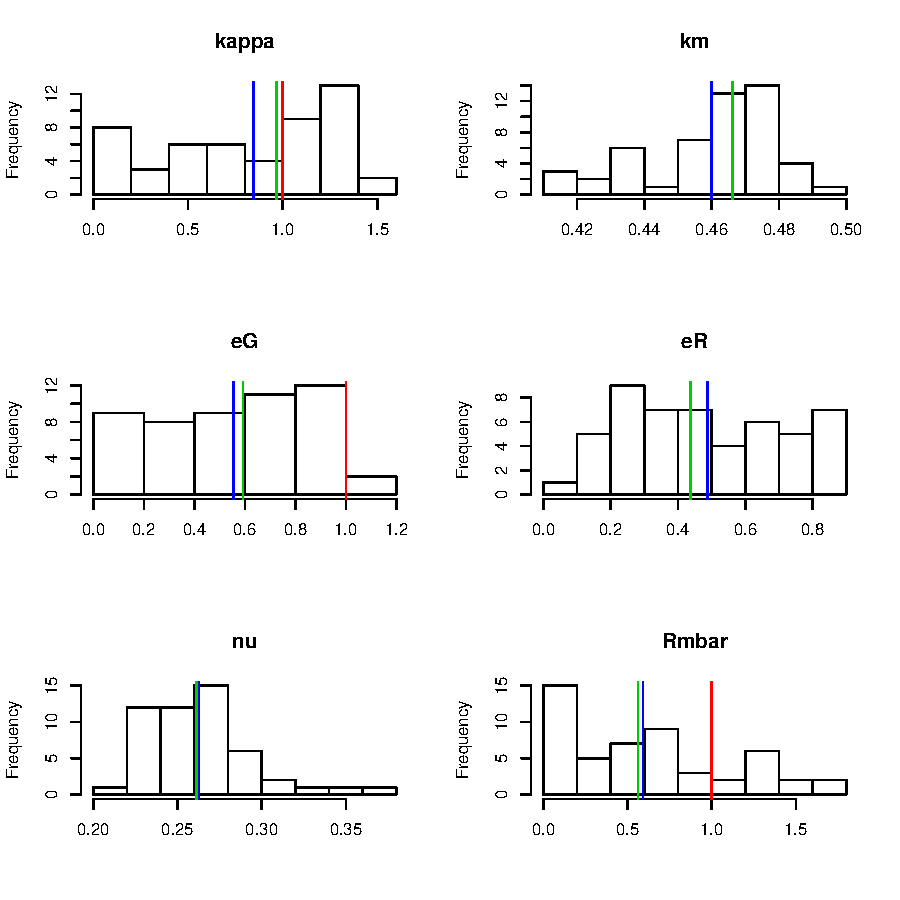
\includegraphics{Solving_the_problem_of_parameter_covariation_4-003}
\end{figure}

None of the parameters are particuarly well-estimated. This differs a
bit from my analysis of the first parameter set, where some of the
parameters were reasonably well-estimated. In particular, the means of
the different parameter estimates were close to the truth. Not so much
here.

Again, I am interested in how well parameter combinations are
estimated. For example, the parameter combination $\kappa/\epsilon_G$
appears in our DEB equations. Is this parameter combination well
estimated, even if $\kappa$ and $\epsilon_G$ are not? No. The true
value of $\kappa/\epsilon_G$ does not even show up on this histogram -
not a single estimate was even in the right ballpark.

\begin{figure}
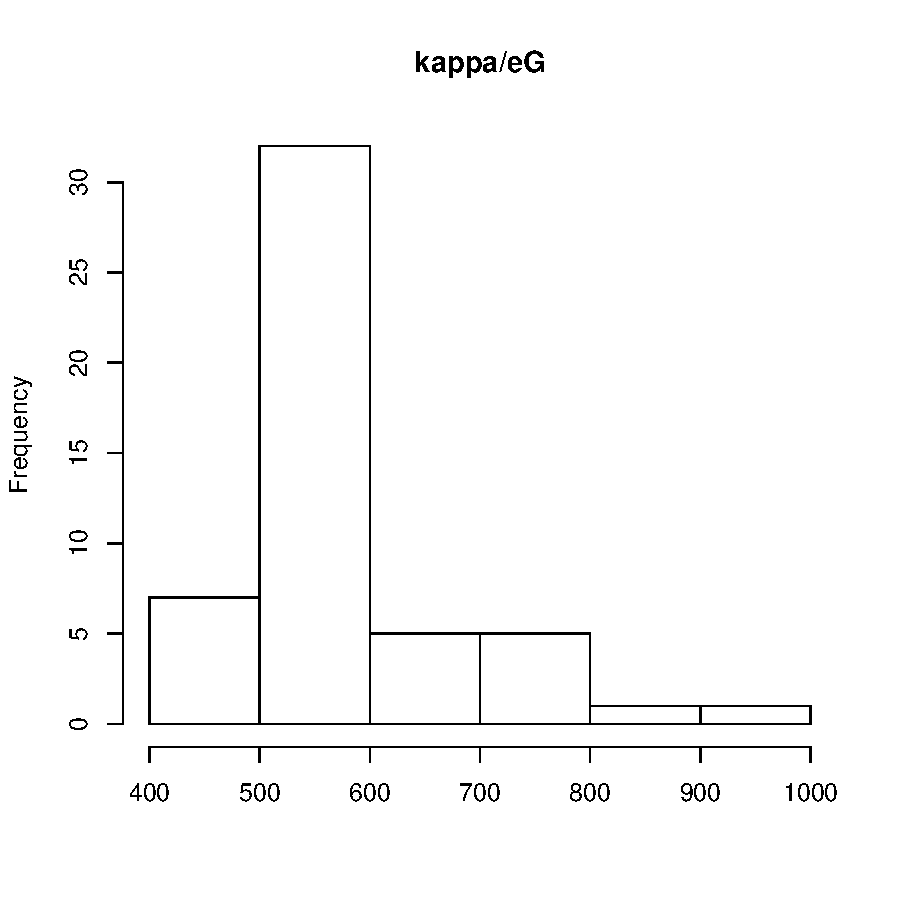
\includegraphics{Solving_the_problem_of_parameter_covariation_4-004}
\end{figure}


\begin{figure}
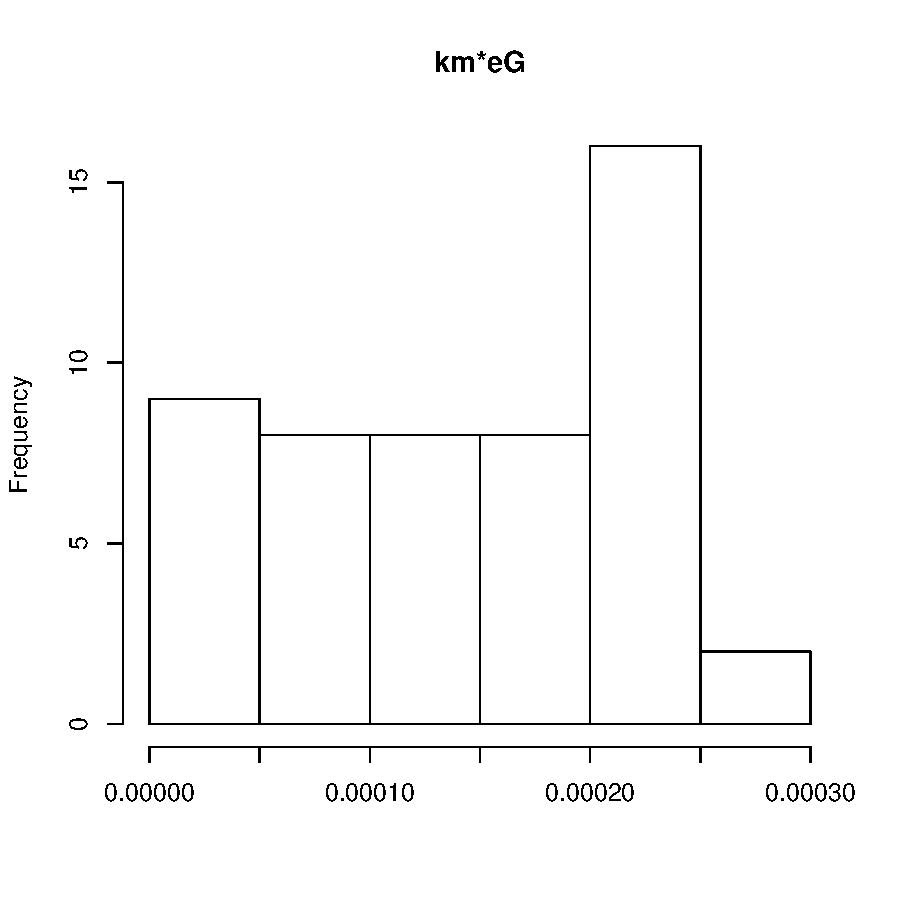
\includegraphics{Solving_the_problem_of_parameter_covariation_4-005}
\caption{Another parameter combination that was well-estimated in the fitting
of the first parameter set, but is not well-estimated now, is $k_m
\epsilon_G$.}
\end{figure}

\begin{figure}
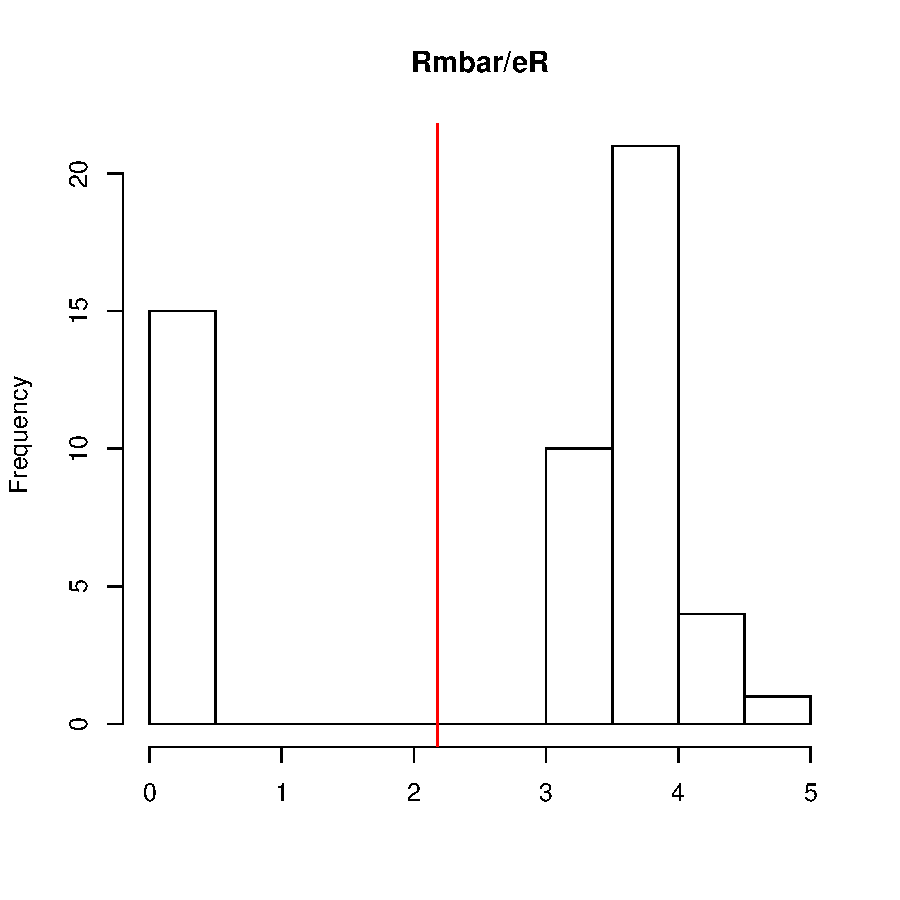
\includegraphics{Solving_the_problem_of_parameter_covariation_4-006}
\caption{The ratio $\bar{R_m}$/$e_R$ was also previously well-estimated, and
now, not so much.}
\end{figure}


\begin{figure}
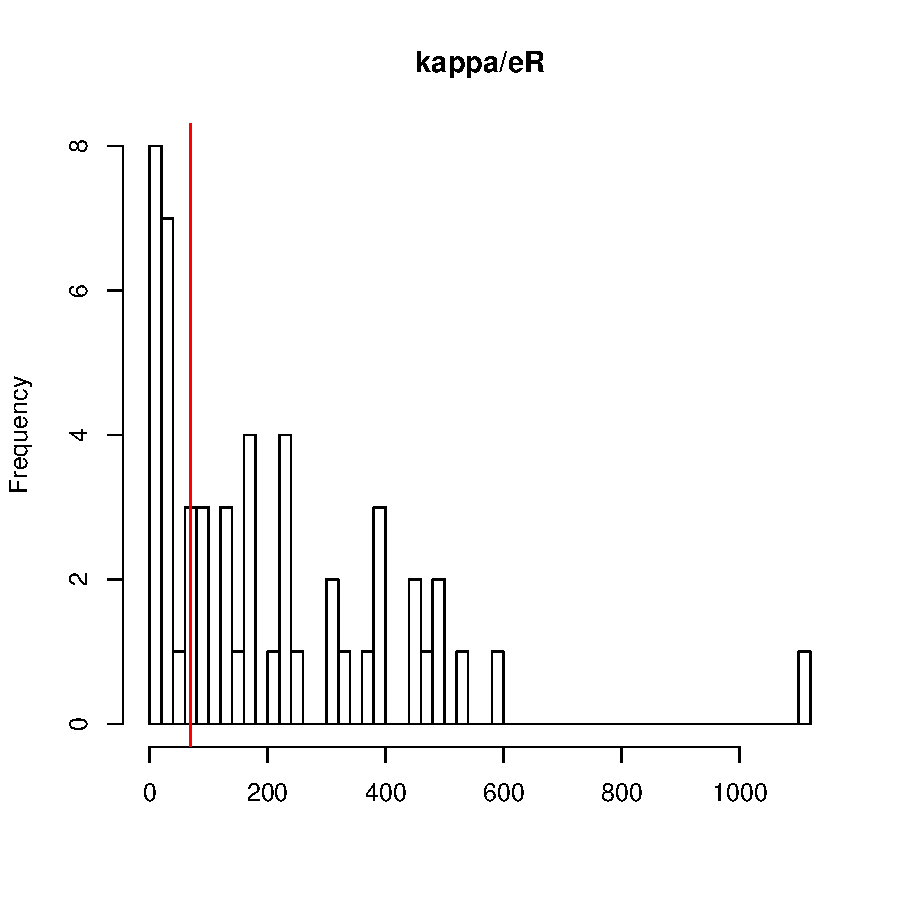
\includegraphics{Solving_the_problem_of_parameter_covariation_4-007}
\caption{$\kappa/\epsilon_R$ is actually pretty well-estimated.}
\end{figure}

All of this is making me wonder whether it might not be better to
combine more than two parameters at the same time. In particular, I
wonder if the non-dimensionalized parameters that Bill and I were
playing around with might not be well-estimated too.

DEB theory makes use of a number of compound parameters - are any of
these well-estimated?

\begin{figure}
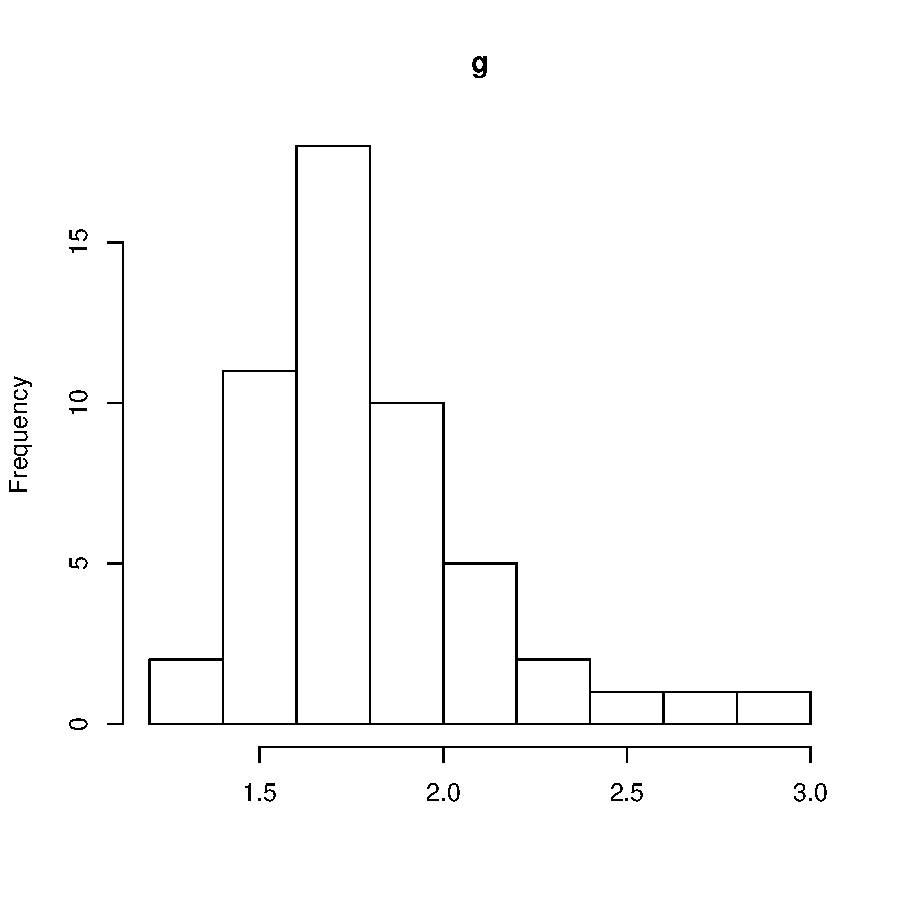
\includegraphics{Solving_the_problem_of_parameter_covariation_4-008}
\caption{Estimates of the DEB compound parameter $g =
  \frac{\epsilon_G \nu}{\kappa p_{am}}$, the energy investment
  ratio.}
\end{figure}

\begin{figure}
\begin{Schunk}
\begin{Sinput}
> hist(res[,'pam']/res[,'nu'],
+      main='Em', xlab='')
> abline(v=true.pars['pam']/true.pars['nu'],col=2)
\end{Sinput}
\end{Schunk}
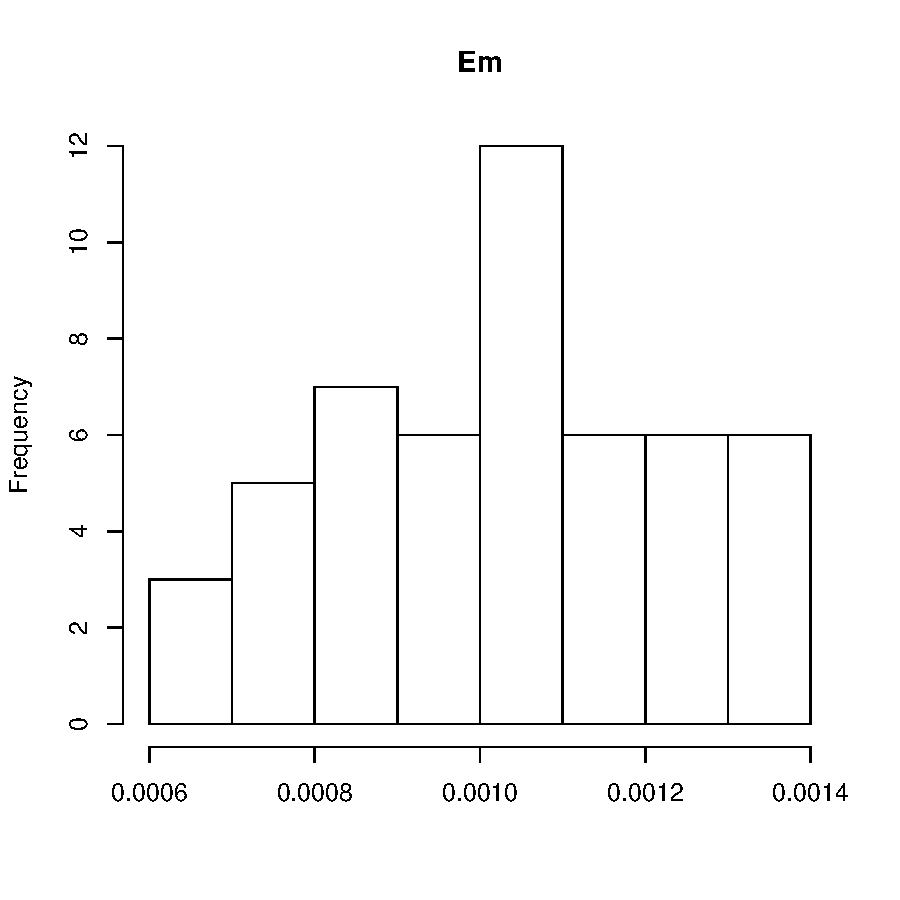
\includegraphics{Solving_the_problem_of_parameter_covariation_4-009}
\caption{Estimates of the DEB compound parameter $E_m = p_{am}/\nu$,
  the maximum reserve density. I'm beginning to wonder if the
  parameter set used to generate the observed data is different from
  the one saved in ``true\_parameters.rda'', given that the parameters
  seem to be converging to something, just not the truth.}
\end{figure}

\begin{figure}
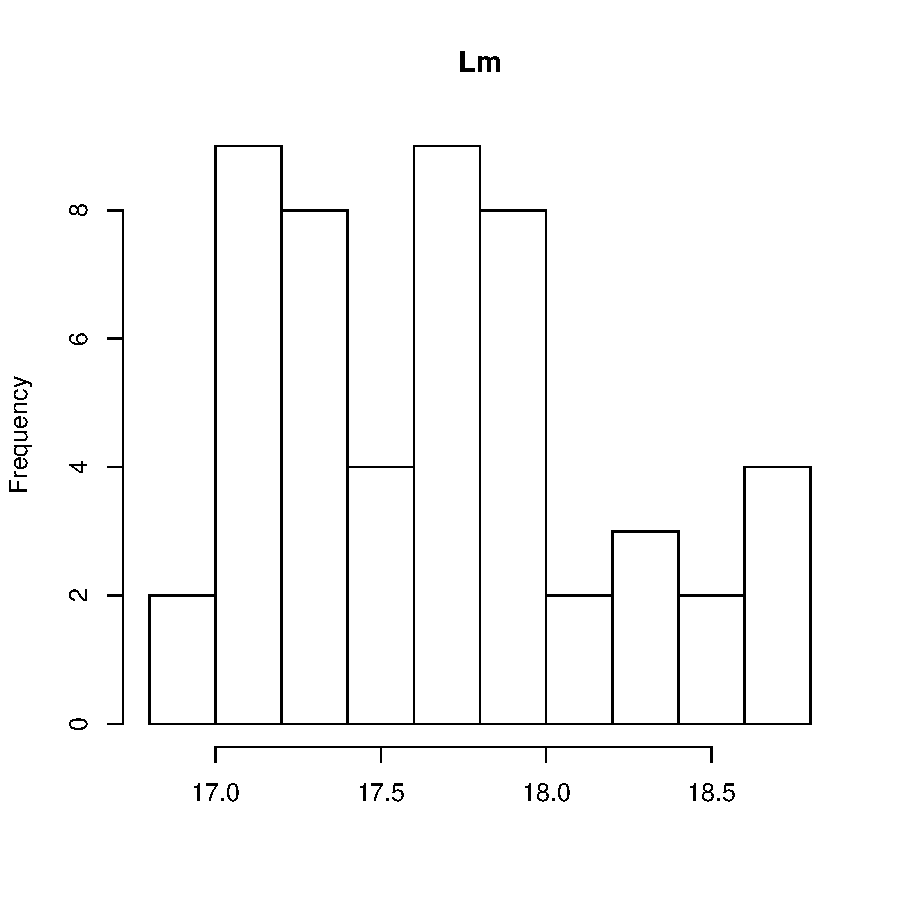
\includegraphics{Solving_the_problem_of_parameter_covariation_4-010}
\caption{Estimates of the DEB compound parameter $L_m = \frac{\kappa
    p_{am}}{k_m \epsilon_G}$, the maximum length. The truth doesn't
  even show up on the histogram.}
\end{figure}

\end{document}
